%!TEX TS-program = xelatex
\documentclass[12pt, a4paper]{article}  
\usepackage{etex} % расширение классического tex в частности позволяет подгружать гораздо больше пакетов, чем мы и займёмся далее

%%%%%%%%%% Математика %%%%%%%%%%
\usepackage{amsmath,amsfonts,amssymb,amsthm,mathtools} 

%%%%%%%%%%%%%%%%%%%%%%%% Шрифты %%%%%%%%%%%%%%%%%%%%%%%%%%%%%%%%%
\usepackage{fontspec}         % пакет для подгрузки шрифтов
\setmainfont{Arial}   % задаёт основной шрифт документа
\defaultfontfeatures{Mapping=tex-text}
\newfontfamily{\cyrillicfonttt}{Arial}
\newfontfamily{\cyrillicfont}{Arial}
\newfontfamily{\cyrillicfontsf}{Arial}
\usepackage{unicode-math}     % пакет для установки математического шрифта
\setmathfont{Asana Math}      % шрифт для математики
\usepackage{polyglossia}      % Пакет, который позволяет подгружать русские буквы
\setdefaultlanguage{russian}  % Основной язык документа
\setotherlanguage{english}    % Второстепенный язык документа

%%%%%%%%%% Работа с картинками %%%%%%%%%
\usepackage{graphicx}                  % Для вставки рисунков
\usepackage{graphics}
\graphicspath{{images/}{pictures/}}    % можно указать папки с картинками

%%%%%%%%%% Графика и рисование %%%%%%%%%%
\usepackage{tikz, pgfplots}  % язык для рисования графики из latex'a
\usepackage{amscd}                  %Пакеты для рисования
\usepackage[matrix,arrow,curve]{xy} %комунитативных диаграмм

%%%%%%%%%% Свои команды %%%%%%%%%%
\usepackage{etoolbox}    % логические операторы для своих макросов
\usepackage{xparse}      % больше команд для создания команд
\usepackage{indentfirst} % Пакет, который ставит в каждом первом абзаце главы красную строку
\setkeys{russian}{babelshorthands=true}

\pgfplotsset{compat=1.13}
\DeclareMathOperator{\Var}{Var}
\DeclareMathOperator{\Cov}{Cov}
\def \s{\ensuremath{\sigma}} 
\newcommand{\xdots}{\ensuremath{x_1 \ldots x_n}}
\newcommand{\com}[2]{\ensuremath{x_{#1} \ldots x_{#2}}}
\renewcommand{\labelitemi}{\textcolor{blue}{$\bullet$}}
\newcommand{\llim}[3]{\lim\limits_{{#1}\to {#2}}{#3}}
\renewcommand{\thefigure}{\thesection:\arabic{figure}}
\renewcommand{\theequation}{Eq.(\arabic{figure})}
\newcommand{\povorot}[2]{\raisebox{\depth}{\scalebox{#1}[-1]{#2}}}


\author{Кунакбаева Камила}
\title{Задание 1}
\date{\today}

\begin{document}

\maketitle

\section{Команды}

$\Cov(X,X)=\Var(X)$.

Чтобы почувствовать разницу: Var $Var$ $\Var$.

\s -алгебра удобнее, чем $\sigma$-алгебра.

\xdots

\com{a}{z}

\com{1}{6}

\com{(a,b)}{(c,d)}

\section{Пункты}

\begin{itemize}
\item \textit{Первый пункт}
\item \textit{Второй пункт}
\item \textit{Третий пункт}
\item \textit{Четвертый пункт}
\end{itemize}

\section{Пределы}

Предел нормальный и в тексте: $\llim{n}{\infty}{\frac{n+1}{n}}$, и вне его:
\[\llim{n}{\infty}{\frac{n+1}{n}}\]

\section{Рисунок}

Дискотека математика.

\begin{figure}[h]
\label{pic:1}
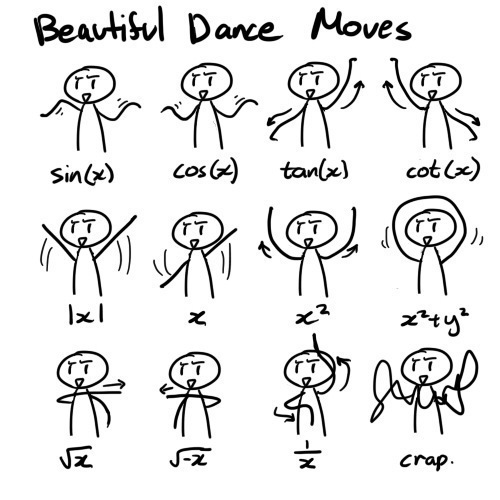
\includegraphics[scale=0.5]{dance.jpg}
\caption{Танец}
\end{figure}

\section{Формулы}

\begin{equation}\label{eq:f1}
2 \cdot 2 = 4,
\end{equation}

Да, мне лень было вбивать сложную формулу, поэтому использовала это:\eqref{eq:f1}.

\section{Перевертыш}

\povorot{1}{Перевернись!}

\povorot{-1}{Перевернись!}
%\povorot{"1" - не поворачивает зеркально, "-1" - поворачивает}{текст}

\end{document}